\chapter{Input and Output} % (fold)
\label{cha:input_and_output}

\begin{quote}
  \Fontlukas\Large
  \renewcommand{\LettrineTextFont}{\relax}
  \lettrine[image=true,lines=3,lraise=0.1]
  {Y}{ou} are progressing well. You have already mastered most of the basics of spell and potion craft, so now we can turn our attention to the creation of scrolls. These magical devices will allow you to capture the magical energies created in your spells, and store them to be retrieved at a later time. Gather your parchment and wand, now summon the energies for your spell and \ldots
\end{quote}

\bigskip

Over the previous chapter you have leant to create programs that manipulate data. So far this data has only existed within the program, with the values stored being lost when the program terminates. If you want to be able to maintain these values between executions you need to learn to save data to file. By saving the program's data to file you can then load it back in when the program is restarted.

This chapter will introduce the artefacts needed to save data from your program to file, and to load that data from file. Using this you will be able to persist data, making it available to future executions of the program.

When you have understood the material in this chapter you will be able to save and load data from text and binary files. 

\clearpage

\minitoc

\clearpage
\section{Input and Output Concepts} % (fold)
\label{sec:input_and_output_concepts}

\clearpage
\subsection{Persisting Data} % (fold)
\label{sub:persisting_data}

When a program is running it uses variables and dynamically allocated memory to store the data it requires. These values exist within the memory allocated to the program when it was started. When the program ends its allocated memory is released, and the values stored within the program are lost. If values must be \emph{remembered} between executions then this data must be stored outside of the program. To achieve this you can save data from the program into files that are stored on the computer's hard drive or solid state drive (SSD).

\begin{figure}[h]
   \centering
   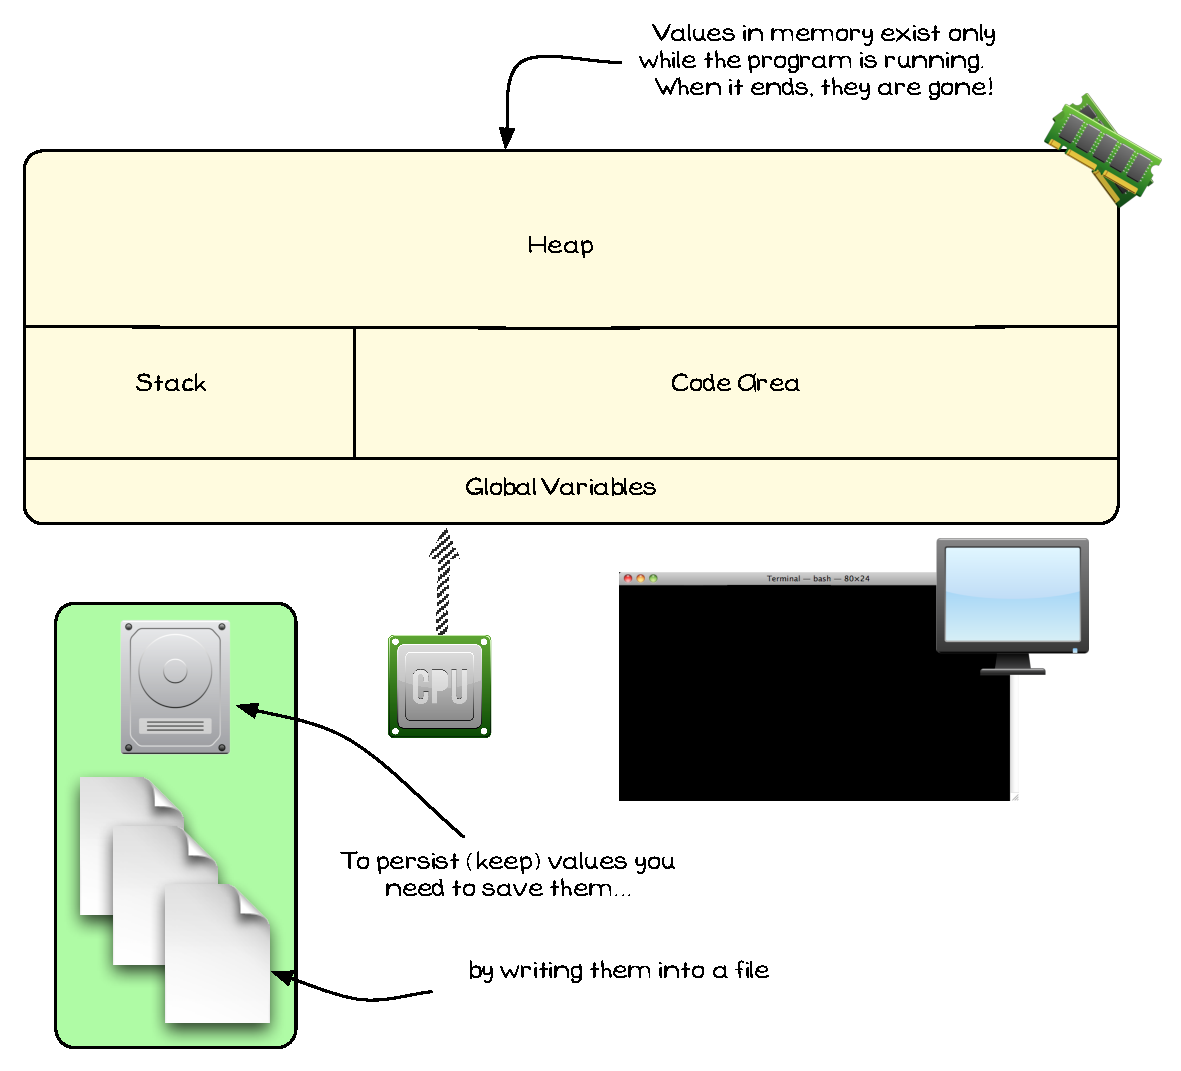
\includegraphics[width=\textwidth]{./topics/file-io/diagrams/PersistData} 
   \caption{When a program ends its data is gone, unless you save it to file}
   \label{fig:persist-data}
\end{figure}

\mynote{
\begin{itemize}
  \item Data stored within a program is lost when the program ends.
  \item To \emph{remember} data between executions it must be saved to file.
  \item The files are stored in a persistent way on a hard drive, or solid state drive.
  \item Hard drives, and solid state drives, are as data storage devices to persist data needed by programs on the computer.
\end{itemize}
}

% subsection persisting_data (end)
\clearpage
\subsection{Interacting with Files} % (fold)
\label{sub:interacting_with_files}

Programming languages offer a number of functions and procedures that are used to interact with files. These will allow you to save data to a file, and load data back from the file.

\begin{figure}[h]
   \centering
   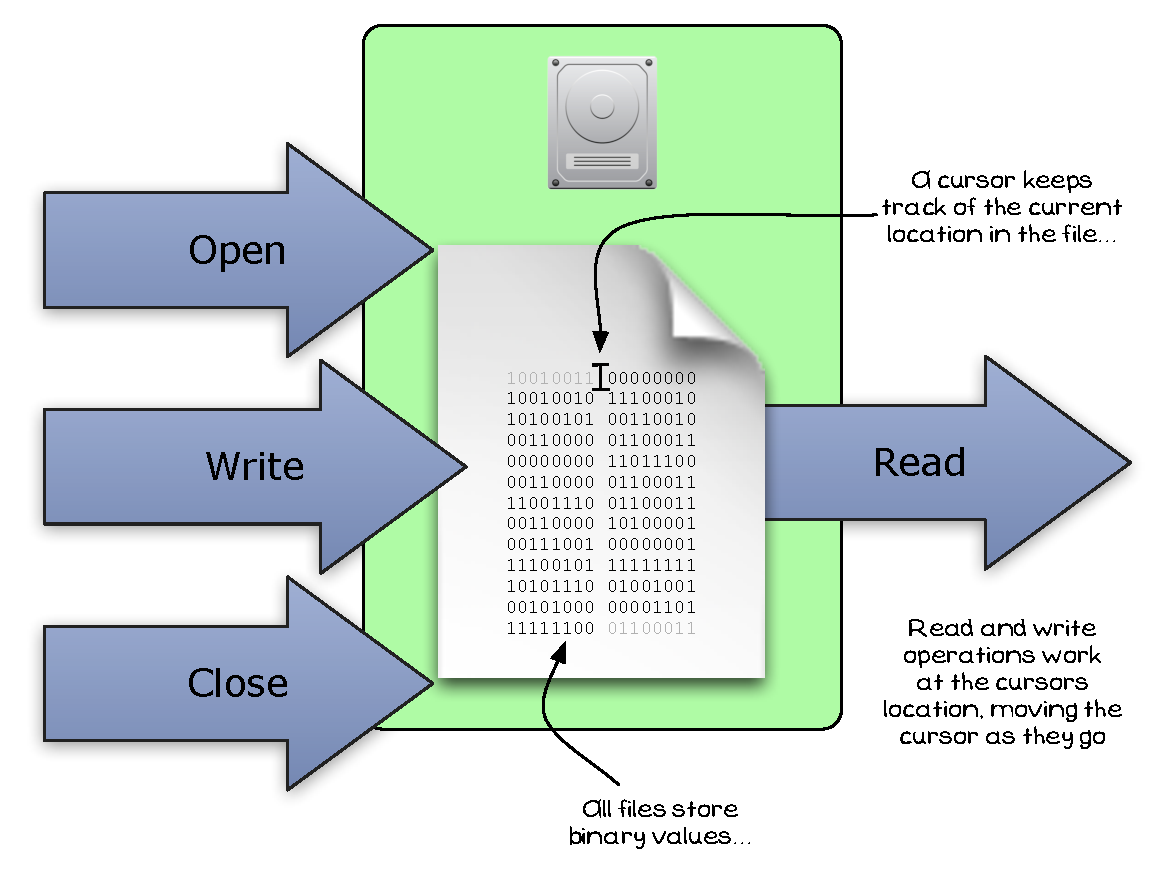
\includegraphics[width=\textwidth]{./topics/file-io/diagrams/FileOps} 
   \caption{File operations include the ability to open, read, write, and close files}
   \label{fig:file-ops}
\end{figure}

\mynote{
\begin{itemize}
  \item Programming languages will provide functions and procedures to:
  \begin{itemize}
    \item \textbf{Open} a file so you can interact with its contents.
    \item \textbf{Read} data from a file that has been opened to be read.
    \item \textbf{Write} data to a file that has been opened to be written to.
    \item \textbf{Close} a file that is currently open.
  \end{itemize}
  \item Languages will also provide built in file types that are used with these functions and procedures.
  \item When you open a file you indicate if you want read and/or write access to its contents.
  \item Opening a file gives you access to a cursor that you can use to read data from the file, or write data to the file.
  \item Standard usage will be to open the file, read/write data to the file, and then close the file.
\end{itemize}
}


% subsection interacting_with_files (end)
\clearpage
\subsection{File Formats} % (fold)
\label{sub:file_formats}

There are two main file formats that you can work with in your program: binary files and text files. A text file stores its data as textual characters, whereas a binary file stores the values directly in the file. 

\begin{figure}[h]
   \centering
   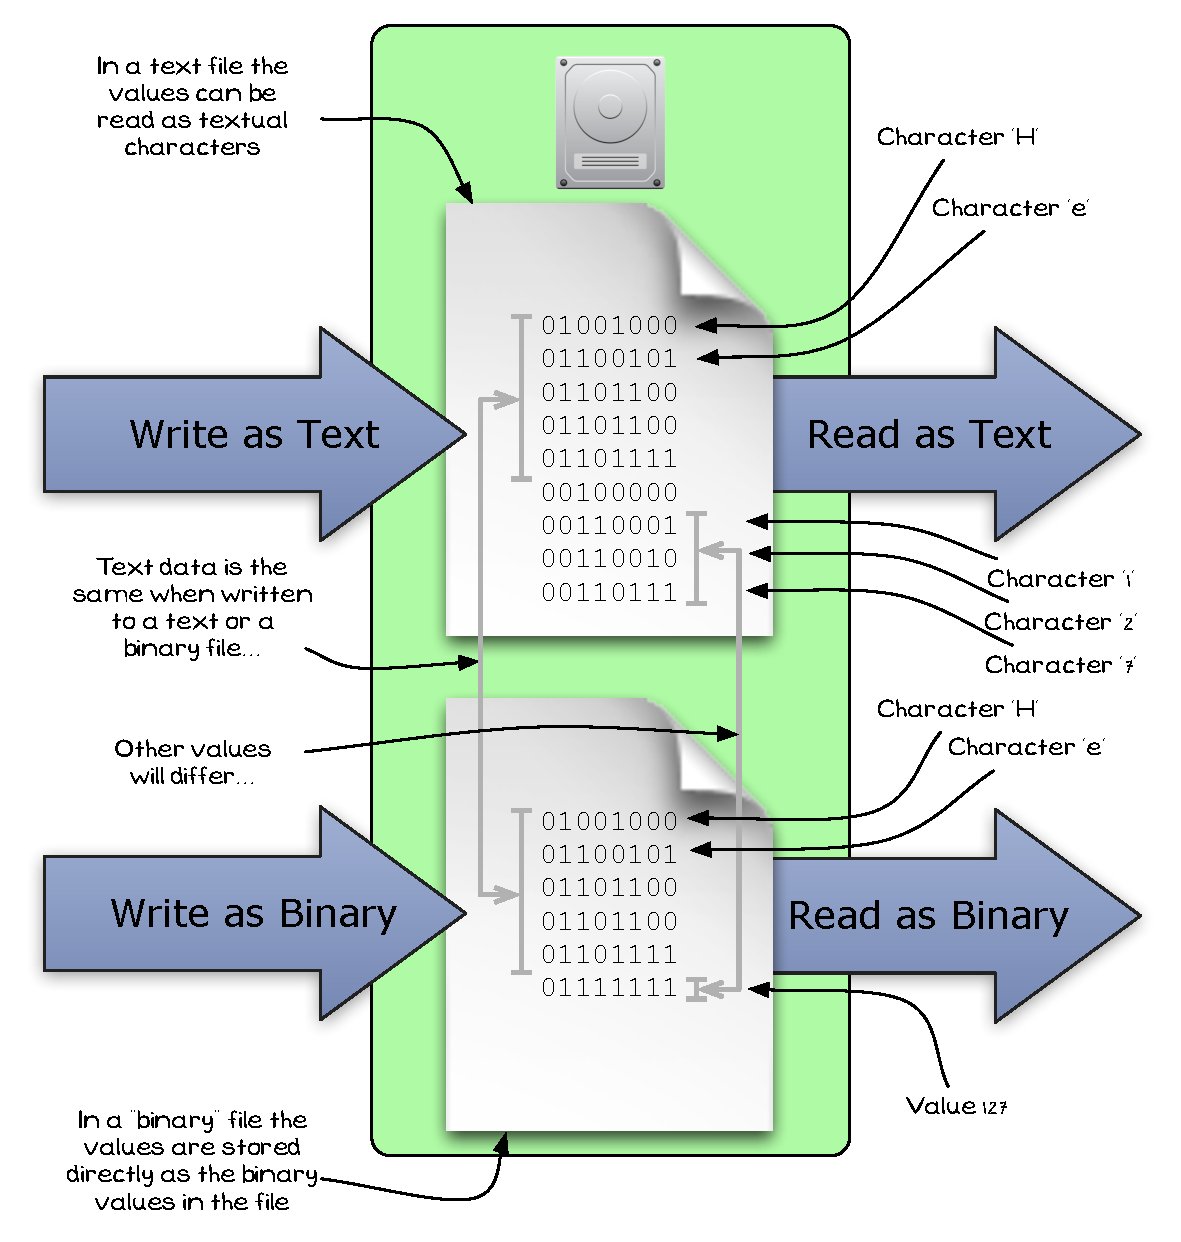
\includegraphics[width=0.9\textwidth]{./topics/file-io/diagrams/FileFormats} 
   \caption{Files can store \emph{textual} or binary data}
   \label{fig:file-formats}
\end{figure}

\mynote{
\begin{itemize}
  \item \fref{fig:file-formats} shows a binary and text file used to save the text `Hello' and the integer 127.
  \item In the \emph{text} file they are stored as the characters `H', `e', `l', `l', `o', and `1', `2', and `7' separated by a space.
  \item In the \emph{binary} file the characters are stored in the same way (as they are text), but the integer is stored as the value 127 which if interpreted as text is a \emph{delete} character.
  \item If you opened these files in a text editor you could read the values from the text file, but you would see a strange character instead of the number 127 in the binary file.
\end{itemize}
}


% subsection file_formats (end)
\clearpage
\subsection{File Structures} % (fold)
\label{sub:file_structures}

When thinking about using using files, the one aspect that you need to spend the most time on will be the organisation of the data in the file. You need to ensure that the data you save includes sufficient information that it can be read back into the program at a later stage. Some common strategies are to:

\begin{enumerate}
  \item Write fixed size data blocks where possible.
  \item Store meta data\footnote{Meta data is data about your data.}, such as the number or size of variable data blocks.
  \item Alternatively, mark the end of variable sized or numbered data blocks with a \emph{sentinel} values.
\end{enumerate}

\begin{figure}[h]
   \centering
   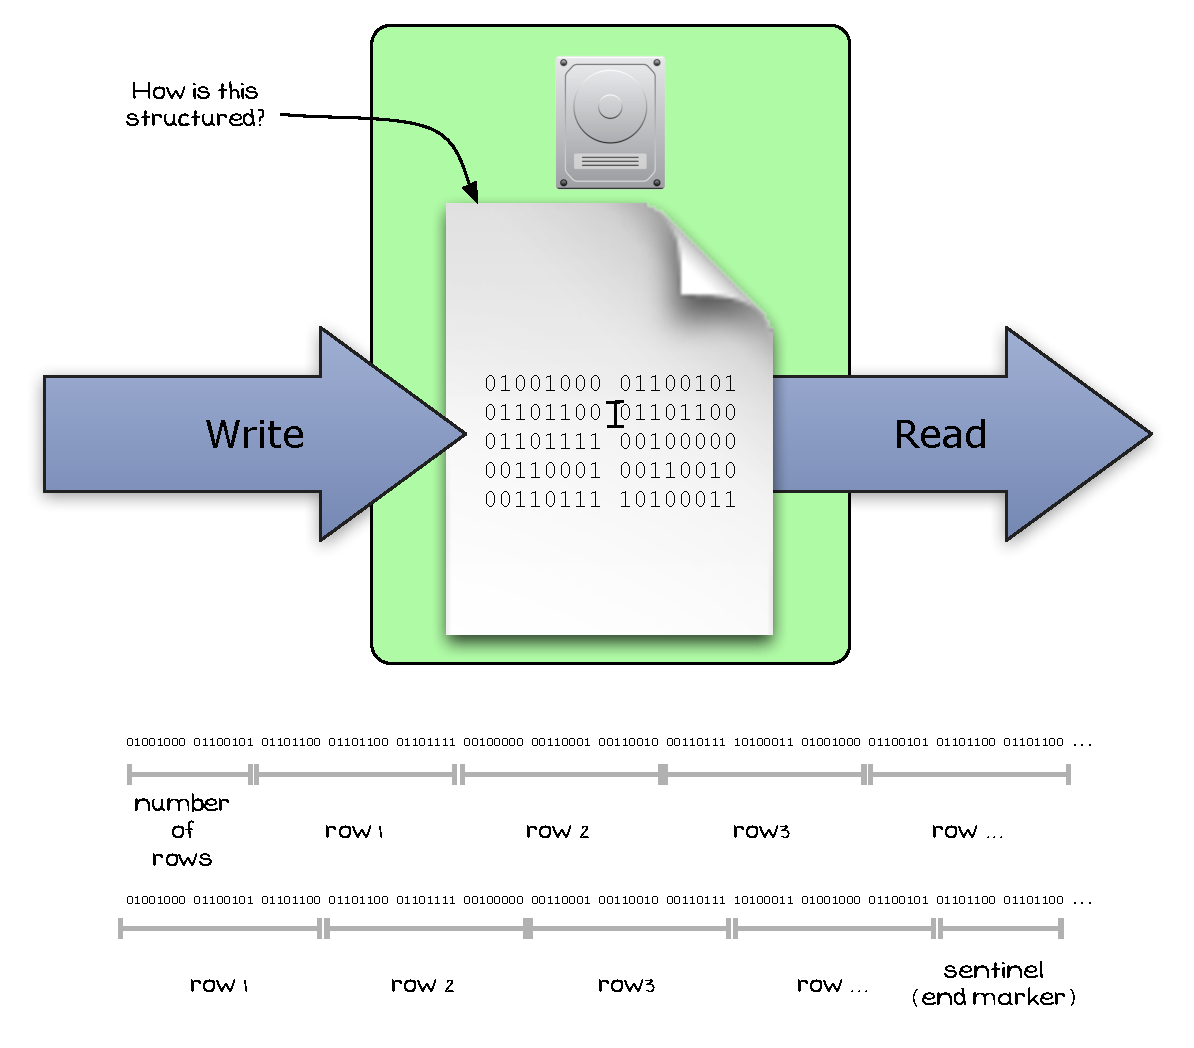
\includegraphics[width=0.9\textwidth]{./topics/file-io/diagrams/FileStructures} 
   \caption{You need to structure data within the file to make it possible to read back successfully.}
   \label{fig:file-structures}
\end{figure}

\mynote{
\begin{itemize}
  \item \fref{fig:file-structures} shows different ways of structuring a variable number of `row' values within a file.
  \item The row values are fixed size blocks, or use their own strategy to manage variable length data.
  \item One version stores the number of elements in the data before storing the data itself.
  \item An alternate strategy is to store a sentinel value at the end of the variable length data.\footnote{There is an end of file marker that can also be used for this purpose.}
\end{itemize}
}

% subsection file_structures (end)
\clearpage
\subsection{Other Devices} % (fold)
\label{sub:other_devices}

The input/output operations are fairly standardised across different device types. Saving data to a file is very similar to writing it to the Terminal or to a network. The skills you learn with any one of these will be transferable to other devices.

\begin{figure}[h]
   \centering
   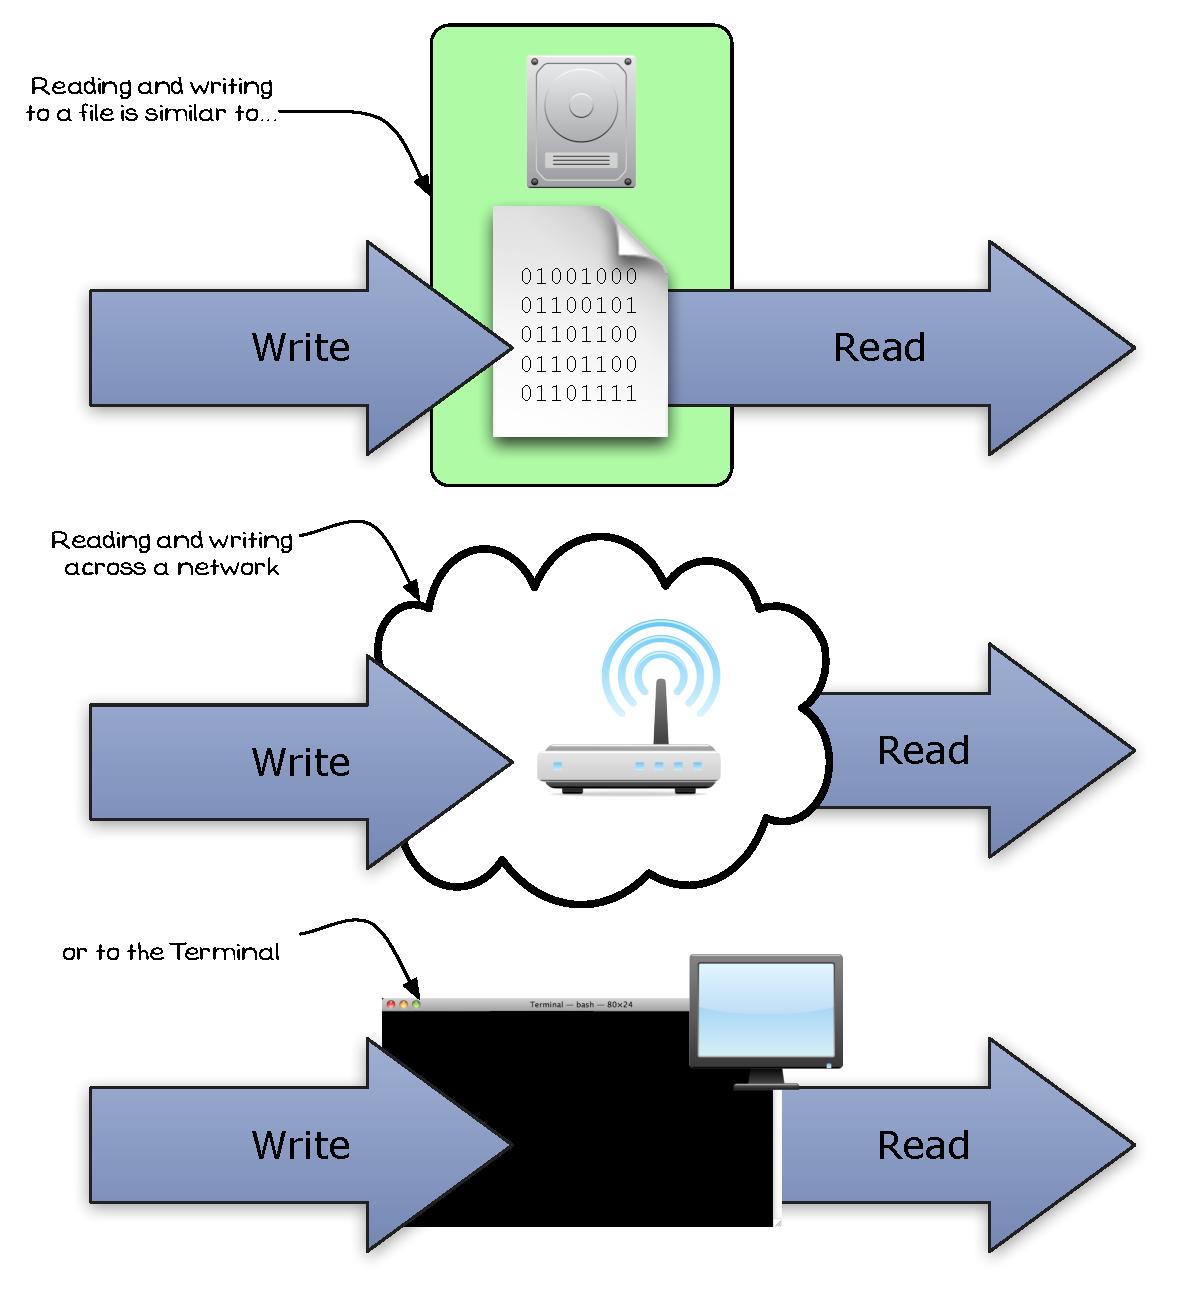
\includegraphics[width=0.9\textwidth]{./topics/file-io/diagrams/OtherDevices} 
   \caption{Writing to other devices also follows similar patterns}
   \label{fig:other-devices}
\end{figure}

\mynote{
\begin{itemize}
  \item The tasks you need to do to read and write data are similar, regardless of the destination device.
  \item Reading and writing to file is similar to reading and writing from the Terminal.
  \item You can open connections to other machines, and read and write data across these connections. Lookup details on sockets if you are interested in doing this.
\end{itemize}
}


% subsection other_devices (end)

% section input_and_output_concepts (end)


\clearpage
\section{Using Input and Output} % (fold)
\label{sec:using_input_and_output}

Using File Input and Output it is now possible to load and save data. As an example we will examine how you can go about saving and loading data in the small db program.

\subsection{Saving Data from Small DB} % (fold)
\label{ssub:saving_data_from_small_db}

The Small DB\footnote{In this chapter we will be saving data from the array based version of the Small DB program, though a similar approach would be taken to save the linked version.} program allows the user to enter a number of \emph{row} values, with each row having a single column that stores a data value (either an integer, text, or double value). At this stage the program only keeps its data while it is executing, once it ends the data is gone. The first step is therefore to save the data from the program into a file.

\subsubsection{Row File Format} % (fold)
\label{ssub:row_file_format}

When thinking about saving data the first task is to try to determine how the data can be saved so that it can later be read back into the program. The following information can help us design the structure of the file saved from the program: 

\begin{enumerate}
  \item There are a variable number of rows.
  \item Each row has a fixed size, when you know the kind of data it is storing.
\end{enumerate}

In this array based version of the Small DB program the number of rows is saved in the \texttt{data store}. This means that an easy way to handle this will be to save the number of rows at the start of the file. This will mean that when the file is loaded back the program can read the number of rows in the file, and create enough space for these in memory before reading them from the file. The pseudocode for save is shown in \lref{plst:save}.

\pseudocode{plst:save}{Pseudocode for Save (for Small DB array version)}{topics/file-io/application/save_data_store.txt}

\mynote{
\begin{itemize}
  \item Notice the number of rows is saved first.
  \item Following this each row is saved to the file.
\end{itemize}
}

The \texttt{Save} procedure calls a \texttt{Save Row} procedure to save each individual row to the file. The pseudocode for this is shown in \lref{plst:save_row}. This code saves the \texttt{id} and \texttt{kind} values to the file, and then uses a \nameref{sub:case_statement} select whether to output the integer value, double value, or text value from the \texttt{row}'s data.

\pseudocode{plst:save_row}{Pseudocode for Save Row (for Small DB array version)}{topics/file-io/application/save_row.txt}

% subsubsection row_file_format (end)


% subsection saving_data_from_small_db (end)

% section using_input_and_output (end)


\clearpage
\def\pageLang{c}

\section{Input and Output in C} % (fold)
\label{sec:file_io_in_c}

\subsection{Implementing Small DB File IO in C} % (fold)
\label{sub:implementing_small_db_file_io_in_c}

\sref{sec:using_input_and_output} presented an altered version of the Small DB program from \cref{cha:dynamic_memory_allocation}. The changes introduced four new procedures used to save the programs data to file, and to reload the data from file. The new code is presented in \lref{lst:c-small-db3}.

\straightcode{\ccode{lst:c-small-db3}{New C code for the Small DB program with file loading and saving}{code/c/file-io/small-db-changes.c}}

\mynote{
\begin{itemize}
  \item The \texttt{FILE} type is used to refer to files that have been opened for the application. See \sref{sub:c_file_type} \nameref{sub:c_file_type}.
  \item 
\end{itemize}
}

% subsection implementing_small_db_file_io_in_c (end)
\clearpage

\subsection{C File Type} % (fold)
\label{sub:c_file_type}

C includes a \texttt{FILE} type that is used to interact with files on the computer. This type includes all of the information that C needs to read and write data to a file. 

\csection{\ccode{clst:file}{Example use of the FILE type to read and write text data}{code/c/file-io/text-file-io.c}}

\mynote{
\begin{itemize}
  \item The \texttt{FILE} type is used to read and write data from a file.
  \item You open the file using \texttt{fopen}.
  \item After the file has been opened you must remember to close it using \texttt{fclose}.
  \item File based versions of \texttt{printf} and \texttt{scanf} allow you to read and write data from the file.
  \item The IO code in C always works with \texttt{FILE} pointers, as a result all of your \texttt{FILE} variables will be pointers.
\end{itemize}
}


% subsection c_file_type (end)
\clearpage
\subsection{C File Functions} % (fold)
\label{sub:c_file_functions}

There are a number of functions and procedures in the \textbf{stdio.h} header that will give you the ability to read and write data from files.

\subsubsection{Opening a file} % (fold)
\label{ssub:opening_a_file}

Before you can interact with a file the first step will be to open the file. This is done with the \texttt{fopen} function. This function will return a FILE pointer you can then use to interact with the file.

\begin{table}[h]
  \centering
  \begin{tabular}{|c|p{9.5cm}|}
    \hline
    \multicolumn{2}{|c|}{\textbf{Function Prototype}} \\
    \hline
    \multicolumn{2}{|c|}{} \\
    \multicolumn{2}{|c|}{\texttt{FILE *fopen( const char *filename, const char *mode )}} \\
    \multicolumn{2}{|c|}{} \\
    \hline
    \multicolumn{2}{|c|}{\textbf{Returns}} \\
    \hline
    \texttt{FILE *} & If successful this returns a pointer to the file stream opened, otherwise it returns NULL. \\
    \hline
    \textbf{Parameter} & \textbf{Description} \\
    \hline
    \texttt{ filename } & The name of the file to open. This can include a relative or absolute path to the file. \\
    & \\
    \texttt{ mode } & Indicates the kind of operations that can be performed on the file. Mode should be one of the following:\\
    & 
    \begin{tabular}{|l|p{7cm}|}
      \hline
      \textbf{mode} & \textbf{description} \\
      \hline
      \texttt{"r"} & Open the file for reading. The file must exist.\\
      \hline
      \texttt{"w"} & Open the file for writing. This will create a new file, or replace an existing file.\\
      \hline
      \texttt{"a"} & Open the file for appending data. This will append data to an existing file, or create a new file if it does not exist.\\ 
      \hline
      \texttt{"r+"} & Open the file for reading, and writing. The file must exist. \\
      \hline
      \texttt{"w+"} & Open the file for writing, and reading. This will create a new file, replacing any existing files.\\
      \hline
      \texttt{"a+"} & Open the file for appending, and reading. This ensures that all write operations are always performed at the end of the file. \\
     \hline
    \end{tabular}
    
     \\
    \hline
  \end{tabular}
  \caption{Details of the \texttt{fopen} function}
  \label{tbl:fopen}
\end{table}

\mynote{
\begin{itemize}
  \item Remember to check that \texttt{fopen} has returned you a valid pointer, if you get back NULL then it failed to open the file.
  \item For binary files you can append a \texttt{b} to the mode. For example, to open a binary file for reading you use the mode \texttt{"rb"}, to open for writing and reading you use \texttt{"w+b"}.
\end{itemize}
}

% subsubsection opening_a_file (end)

\clearpage
\subsubsection{Closing a file} % (fold)
\label{ssub:closing_a_file}

Once you have opened a file it is important that you also close it. The \texttt{fclose} function can be used to close an opened file.

\begin{table}[h]
  \centering
  \begin{tabular}{|c|p{9.5cm}|}
    \hline
    \multicolumn{2}{|c|}{\textbf{Function Prototype}} \\
    \hline
    \multicolumn{2}{|c|}{} \\
    \multicolumn{2}{|c|}{\texttt{int fclose( FILE *stream )}} \\
    \multicolumn{2}{|c|}{} \\
    \hline
    \multicolumn{2}{|c|}{\textbf{Returns}} \\
    \hline
    \texttt{int} & Returns 0 when it is successfully closed. \\
    \hline
    \textbf{Parameter} & \textbf{Description} \\
    \hline
    \texttt{ stream } & The file to close. \\
    \hline
  \end{tabular}
  \caption{Details of the \texttt{fclose} function}
  \label{tbl:fclose}
\end{table}

\mynote{
\begin{itemize}
  \item Make sure to close all opened files.
  \item Remember to check all paths through your code.
\end{itemize}
}

% subsubsection closing_a_file (end)

\subsubsection{Writing text data to file} % (fold)
\label{ssub:writing_text_data_to_file}

You can use \texttt{fprintf} to write data to a \texttt{FILE} that has been opened with write capabilities. This works the same as \texttt{printf} and \texttt{sprintf}.

\begin{table}[h]
  \centering
  \begin{tabular}{|c|p{9cm}|}
    \hline
    \multicolumn{2}{|c|}{\textbf{Function Prototype}} \\
    \hline
    \multicolumn{2}{|c|}{} \\
    \multicolumn{2}{|c|}{\texttt{int fprintf(FILE *destination, const char *format, \ldots )}} \\
    \multicolumn{2}{|c|}{} \\
    \hline
    \multicolumn{2}{|c|}{\textbf{Returns}} \\
    \hline
    \texttt{int} & The number of characters written to the \texttt{destination} by \texttt{fprintf}. \\
    \hline
    \textbf{Parameter} & \textbf{Description} \\
    \hline
    \texttt{ destination } & The FILE to write the output into.\\
    & \\
    \texttt{ format } & The text that is to be written to the file. This text may contain format tags to include other values. This is the same as \texttt{printf}, see Figure \ref{csynt:program-creation-format-string} for the syntax of the format tag. \\
    & \\
    \texttt{\ldots}   & Optional values, must have at least as many values as format tags. \\
    \hline
  \end{tabular}
  \caption{Parameters that must be passed to \texttt{fprintf}}
  \label{tbl:fprintf}
\end{table}

\mynote{
\begin{itemize}
  \item This will write the data as text to the file.
  \item The file must be opened with write permissions.
\end{itemize}
}

% subsubsection writing_data_to_file (end)

\clearpage

\subsubsection{Reading text data from file} % (fold)
\label{ssub:reading_text_data_from_file}

Reading text data from a file is similar to reading data from the Terminal or from a string. The \texttt{fprintf} function works in the same way as \texttt{printf} and \texttt{sprintf}, but writes its data to a text file.

\begin{table}[h]
  \centering
  \begin{tabular}{|c|p{9.5cm}|}
    \hline
    \multicolumn{2}{|c|}{\textbf{Function Prototype}} \\
    \hline
    \multicolumn{2}{|c|}{} \\
    \multicolumn{2}{|c|}{\texttt{int fscanf(const char *source, const char *format, \ldots )}} \\
    \multicolumn{2}{|c|}{} \\
    \hline
    \multicolumn{2}{|c|}{\textbf{Returns}} \\
    \hline
    \texttt{int} & The number of values read by \texttt{fscanf}. \\
    \hline
    \textbf{Parameter} & \textbf{Description} \\
    \hline
    \texttt{ source } & The string from which the input is read.\\
    & \\
    \texttt{ format } & The format specifier describing what is to be read from the Terminal. This is the same as with \texttt{scanf}, see \tref{tbl:format specifiers}. \\
    & \\
    \texttt{\ldots}   & The variables into which the values will be read. There must be at least as many variables as format tags in the format specifier. \\
    \hline
  \end{tabular}
  \caption{Parameters that must be passed to \texttt{fscanf}}
  \label{tbl:fscanf}
\end{table}

\mynote{
\begin{itemize}
  \item This will read text data from the file.
  \item The file must be opened with read permissions.
\end{itemize}
}

\csection{\ccode{clst:text_io}{Example code that demonstrates writing a value and reading it back from a text file}{code/c/file-io/text_io.c}}


% subsubsection reading_data_from_file (end)


\subsubsection{Writing binary data to file} % (fold)
\label{ssub:writing_binary_data_to_file}

The \texttt{fwrite} function allows you to write binary data to a file. This requires you to pass a pointer to your data, as well as the size and number of elements you want written.

\begin{table}[h]
  \centering
  \begin{tabular}{|c|p{9cm}|}
    \hline
    \multicolumn{2}{|c|}{\textbf{Function Prototype}} \\
    \hline
    \multicolumn{2}{|c|}{} \\
    \multicolumn{2}{|c|}{\texttt{size\_t fwrite( const void *ptr, size\_t size, size\_t count, FILE *destination)}} \\
    \multicolumn{2}{|c|}{} \\
    \hline
    \multicolumn{2}{|c|}{\textbf{Returns}} \\
    \hline
    \texttt{int} & The number of elements written to the \texttt{destination} by \texttt{fwrite}. If this does not equal the \texttt{count} parameter it indicates an error occurred writing the data to the file.\\
    \hline
    \textbf{Parameter} & \textbf{Description} \\
    \hline
    \texttt{ ptr } & A pointer to the data to be saved to the file.\\
    & \\
    \texttt{ size } & The size of each element to be saved.\\
    & \\
    \texttt{ count } & The number of elements to be saved to the file.\\
    & \\
    \texttt{ destination } & The FILE to write the output into.\\
    & \\
    \hline
  \end{tabular}
  \caption{Parameters that must be passed to \texttt{fwrite}}
  \label{tbl:fwrite}
\end{table}

\mynote{
\begin{itemize}
  \item The file must be opened with write permissions.
  \item This will write the binary data to file from the values pointed to by the \texttt{prt} parameter.
\end{itemize}
}

\csection{\ccode{clst:write_binary}{Example code that writing an array of double values to a binary file.}{code/c/file-io/write_binary.c}}


% subsubsection writing_binary_data_to_file (end)

\clearpage
\subsubsection{Reading binary data from file} % (fold)
\label{ssub:reading_binary_data_from_file}

To read back binary data you need to use \texttt{fread}. This reads back a block of data from the file, and stores it in memory at a location indicated by a pointer.

\begin{table}[h]
  \centering
  \begin{tabular}{|c|p{9cm}|}
    \hline
    \multicolumn{2}{|c|}{\textbf{Function Prototype}} \\
    \hline
    \multicolumn{2}{|c|}{} \\
    \multicolumn{2}{|c|}{\texttt{size\_t fread( void *ptr, size\_t size, size\_t count, FILE *destination)}} \\
    \multicolumn{2}{|c|}{} \\
    \hline
    \multicolumn{2}{|c|}{\textbf{Returns}} \\
    \hline
    \texttt{int} & The number of elements read from the \texttt{destination} by \texttt{fprintf}. If this does not equal the \texttt{count} parameter it indicates an error occurred reading the data from the file.\\
    \hline
    \textbf{Parameter} & \textbf{Description} \\
    \hline
    \texttt{ ptr } & A pointer to the location to store the loaded data. This must be large enough to store the values loaded.\\
    & \\
    \texttt{ size } & The size of each element to be loaded.\\
    & \\
    \texttt{ count } & The number of elements to be loaded from the file.\\
    & \\
    \texttt{ destination } & The FILE to read the data from.\\
    & \\
    \hline
  \end{tabular}
  \caption{Parameters that must be passed to \texttt{fwrite}}
  \label{tbl:fread}
\end{table}

\mynote{
\begin{itemize}
  \item The file must be opened with read permissions.
  \item You must ensure that \texttt{ptr} points to sufficient space to load the data into.
\end{itemize}
}

\begin{figure}[p]
  \csection{\ccode{clst:read_binary}{Example code that reads an array of double values from a binary file.}{code/c/file-io/read_binary.c}}  
\end{figure}


% subsubsection reading_binary_data_from_file (end)

% subsection c_file_functions (end)

% section input_and_output_in_c (end)



% \clearpage
% \section{Input and Output in Pascal} % (fold)
% \def\pageLang{pas}
% \label{sec:file_io_in_pascal}
% 
% % section input_and_output_in_pascal (end)

\clearpage
\def\pageLang{none}
% \section{Understanding Input and Output} % (fold)
% \label{sec:understanding_input_and_output}
% 
% % section understanding_input_and_output (end)
% 
% \clearpage
% \section{Input and Output Examples} % (fold)
% \label{sec:input_and_output_examples}
% 
% % section input_and_output_examples (end)
% 

\clearpage
\section{Input and Output Exercises} % (fold)
\label{sec:input_and_output_exercises}

\subsection{Concept Questions} % (fold)
\label{sub:file-io-concept_questions}

\begin{enumerate}
  \item Why would you want to save data to file?
  \item What are the basic operations that you can perform with files?
  \item What is the difference between a text file and a binary file? Explain. 
  \item What challenges to saving variable sized data to file raise? How can these be addressed?
  \item How is reading and writing to files similar to working with the Terminal?
\end{enumerate}

% subsection concept_questions (end)

\subsection{Code Writing Questions: Applying what you have learnt} % (fold)
\label{sub:code_writing_questions_applying_what_you_have_learnt}

\begin{enumerate}
  \item Write two programs that save three integer values to file, one that saves it to a text file the other to a binary file. Execute the two programs and compare the files created.
  \item Write two programs that read three integer values from file, one that reads them from a text file the other from a binary file. Once the data is loaded into memory have the program output them to the terminal.
  \item Use the code from this chapter to implement saving data for the Small DB program.
  \item Revisit your statistics programs and have it save the values the user enters to file when the programs ends. Once this is working add the code to load the data from the file when the programs starts.
\end{enumerate}

% subsection code_writing_questions_applying_what_you_have_learnt (end)

\subsection{Extension Questions} % (fold)
\label{sub:extension_questions}

\begin{enumerate}
  \item Explore the other file IO functions and procedures offered by the language you are using. See if you can work out how to move the cursor within the file (seek to a new location). Use this to move back and forth within a file reading individual values in response to user input. 
\end{enumerate}

% subsection extension_questions (end)

% section input_and_output_exercises (end)


% chapter input_and_output (end)